%
% This document is free; you can redistribute it and/or modify
% it under the terms of the GNU General Public License as published by
% the Free Software Foundation; either version 2 of the License, or
% (at your option) any later version.
%
% This document is distributed in the hope that it will be useful, but
% WITHOUT ANY WARRANTY; without even the implied warranty of
% MERCHANTABILITY or FITNESS FOR A PARTICULAR PURPOSE.  See the GNU
% General Public License for more details.
%
% You should have received a copy of the GNU General Public License
% along with this document; if not, write to the Free Software
% Foundation, Inc., 51 Franklin Street, Fifth Floor, Boston, MA
% 02110-1301, USA.
%
% Author: Bertoli Marco
%
\chapter{JSIM}
\label{cha:jsim}
\section{Overview}
JSIM analyzes open, closed and mixed queueing networks using a discrete-event simulator \cite{DESimulation}. A sequence of \emph{wizard} windows helps specifying network properties. The simulation engine supports several probability distributions for characterizing service and inter-arrival times, e.g., exponential, hyperexponential, uniform, Erlang and Pareto. Random number generation is based on the Mersenne twister engine \cite{Mersenne}. It is also possible to reproduce a given sequence of random numbers, in order to simulate real workloads from collected
log files. Load-dependent strategies using arbitrary functions of the current queue-length can be specified.

JSIM supports state-independent routing strategies, e.g., Markovian or round robin, as well as state-dependent strategies, e.g., routing to the server with minimum utilization, or
with the shortest response time, or with minimum queue length.

Performance indices like throughputs, utilizations, response times, residence times, queue-lengths are evaluated. The simulation engine supports several extended features
not allowed in product-form models, namely, finite capacity regions (i.e., blocking), fork-join servers, and priority classes. Finite capacity regions may include either shared
or class-specific population constraints. 

The analysis of simulation results employs on-line transient detection techniques based on spectral analysis \cite{Spectral}. What-if analysis, where a sequence of simulations is run for different
values of parameters, are also possible.

\subsection{Starting the alphanumeric simulator}
Selecting 
\includegraphics[scale=.5]{img/JSIMIcon} button on the
starting screen, \autoref{fig:jsim:Classes} window shows up.
\begin{figure}[htb]
    \begin{center}
        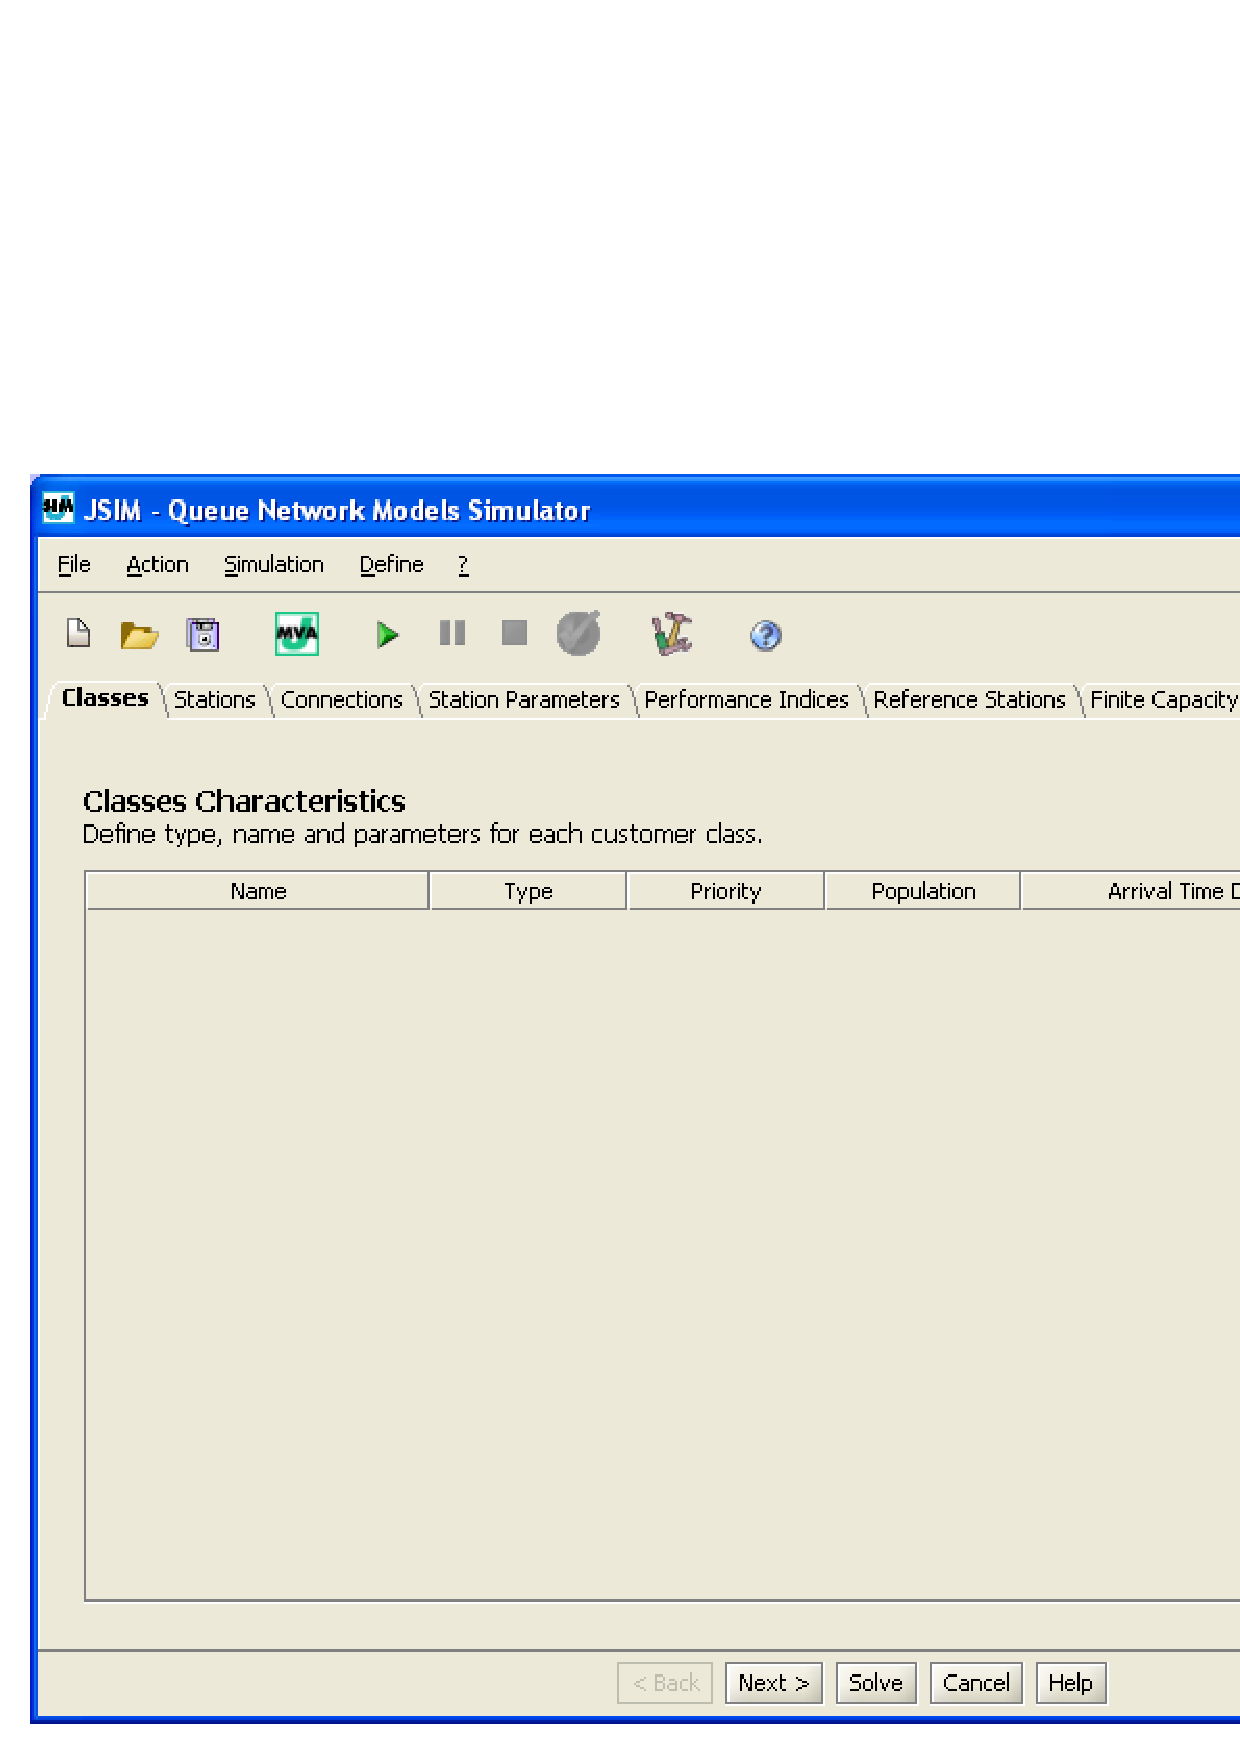
\includegraphics[width=300]{img/jsim/classes}
    \end{center}
    \caption{Classes Panel}
    \label{fig:jsim:Classes}
\end{figure}
Each JSIM panel is organized to be compliant with a given layout, shown in \autoref{fig:jsim:panellayout}, 
\begin{figure}[tb]
    \begin{center}
        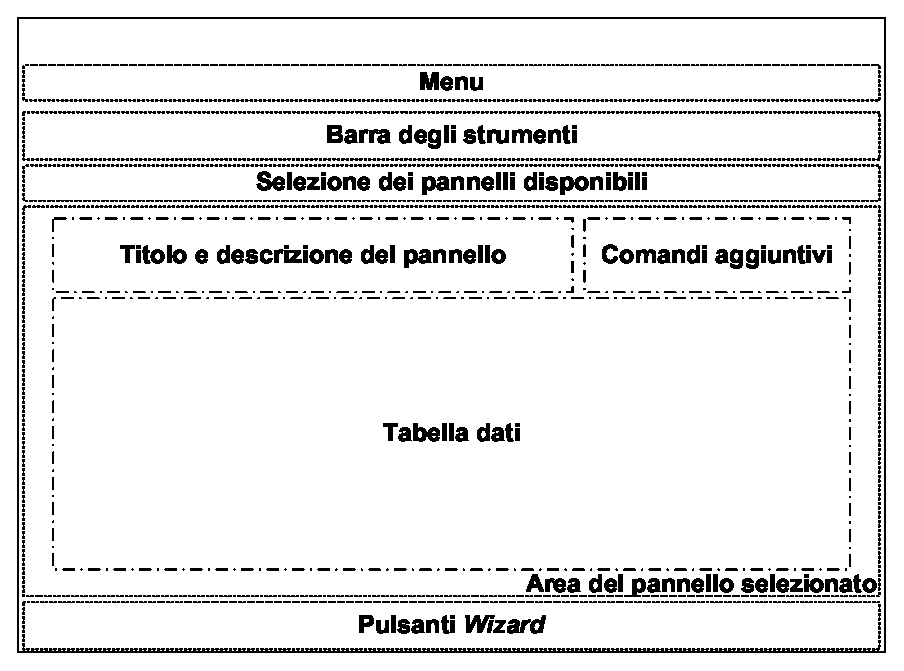
\includegraphics[width=300]{img/jsim/panelLayout}
    \end{center}
    \caption{Layout of JSIM panels}
    \label{fig:jsim:panellayout}
\end{figure}
where the following main areas can be identified:

